% =====================================================================
%  TP2 - Reconstrucción 3D  |  I308 Visión Artificial (UdeSA, 2026)
%  Compilar con pdfLaTeX. Las figuras están en la carpeta img/.
%  Números según la corrida del notebook del commit 85b7b44; malla de Poisson según notebooks/opcional.ipynb.
% =====================================================================
\documentclass[10pt,a4paper,twocolumn]{article}

\usepackage[utf8]{inputenc}
\usepackage[T1]{fontenc}
\usepackage[spanish,es-tabla,es-nodecimaldot,es-noshorthands]{babel}
\usepackage{newtxtext,newtxmath}
\usepackage[top=1.6cm,bottom=1.6cm,left=1.5cm,right=1.5cm,columnsep=0.6cm]{geometry}
\usepackage{graphicx}
\graphicspath{{img/}}
\usepackage{amsmath}
\usepackage{booktabs,multirow}
\usepackage[font=footnotesize,labelfont=bf,skip=3pt]{caption}
\usepackage{subcaption}
\usepackage{xcolor}
\usepackage{microtype}
\usepackage{placeins}    % \FloatBarrier: las figuras de resultados no pasan a la discusión
\usepackage{titlesec}
\usepackage[hidelinks]{hyperref}

% --- espaciado compacto ---------------------------------------------
\titlespacing*{\section}{0pt}{8pt plus 2pt minus 2pt}{3pt}
\titlespacing*{\subsection}{0pt}{6pt plus 1pt minus 1pt}{2pt}
\setlength{\textfloatsep}{8pt plus 2pt minus 2pt}
\setlength{\dbltextfloatsep}{8pt plus 2pt minus 2pt}
\setlength{\intextsep}{8pt plus 2pt minus 2pt}
\setlength{\floatsep}{6pt plus 2pt minus 2pt}
\renewcommand{\topfraction}{0.9}
\renewcommand{\dbltopfraction}{0.9}
\renewcommand{\textfraction}{0.07}
\renewcommand{\floatpagefraction}{0.85}
\renewcommand{\dblfloatpagefraction}{0.85}
\setlength{\parskip}{0pt}
\setlength{\emergencystretch}{2em}   % evita espacios enormes con nombres de función largos
\AtBeginDocument{\setlength{\abovedisplayskip}{4pt}\setlength{\belowdisplayskip}{4pt}\setlength{\abovedisplayshortskip}{2pt}\setlength{\belowdisplayshortskip}{3pt}}

\newcommand{\px}{\,\mathrm{px}}
\newcommand{\mm}{\,\mathrm{mm}}
\newcommand{\T}{^{\top}}
\newcommand{\code}[1]{\texttt{#1}}
\newcommand{\pendiente}[1]{\textcolor{red}{#1}}

\begin{document}

% --- título y resumen (a todo el ancho) ------------------------------
\twocolumn[{%
\begin{center}
  {\LARGE\bfseries Trabajo Práctico 2: Reconstrucción 3D}\\[3pt]
  {\large I308 -- Visión Artificial, Universidad de San Andrés}\\[3pt]
  Luis Embon Strizzi \quad$\cdot$\quad Franco Sandri \quad$\cdot$\quad Alan Yeger\\[2pt]
  {\small Octubre de 2026}
\end{center}
\vspace{-2pt}
\begin{center}
\begin{minipage}{0.93\textwidth}
\small\noindent\textbf{Resumen.}\; Se presenta la reconstrucción tridimensional de un peluche a partir de 27 pares de imágenes tomados con una cámara estéreo en una órbita completa alrededor del objeto, apoyado sobre un tablero ChArUco que define el marco de referencia global. El sistema estéreo se calibró con la herramienta de la cátedra, con un error de reproyección de $1{,}25\px$, y su escala métrica se verificó de forma independiente triangulando las esquinas del tablero, cuyo lado se recupera con un error del $0{,}3$\,\%. Sobre cada par rectificado se calcula un mapa de disparidad con SGBM, cuyos parámetros se ajustaron de forma interactiva con \code{stereodemo} y se compararon con la red neuronal CREStereo. Cada mapa se convierte en una nube de puntos local mediante la matriz de reproyección $Q$, la pose de la cámara se estima con \code{solvePnP} sobre las esquinas del tablero y las nubes se transforman al marco global teniendo en cuenta la rotación introducida por la rectificación. La nube fusionada, de $9{,}3$ millones de puntos, se reduce a unos $176\,000$ mediante filtrado espacial, submuestreo por vóxeles y eliminación de puntos espurios en Open3D. Sobre el resultado se estima un alto de $280\mm$ y un ancho de $294\mm$, con errores relativos del $3{,}5$ y el $2{,}0$\,\% respecto de las medidas reales del objeto. Como paso opcional, se obtuvo además una malla de la superficie mediante la reconstrucción de Poisson.
\end{minipage}
\end{center}
\vspace{4pt}
}]

% =====================================================================
\section{Introducción y marco teórico}
\label{sec:intro}
% =====================================================================

El objetivo del trabajo es obtener la nube de puntos 3D de un objeto a partir de varios pares de imágenes estéreo y estimar sus dimensiones en milímetros. A diferencia de la reconstrucción con una única cámara en movimiento, que recupera la escena sólo salvo un factor de escala, un sistema estéreo calibrado conoce la distancia entre sus dos cámaras y, por lo tanto, mide profundidades en unidades métricas. La reconstrucción completa requiere además observar el objeto desde todos sus lados y expresar cada vista en un marco común, que en este trabajo está dado por un tablero de calibración visible en todas las capturas. En esta sección se resumen los conceptos sobre los que se apoya el pipeline.

\subsection{Modelo de cámara y calibración}
\label{sec:pinhole}

En el modelo \emph{pinhole}, un punto $\mathbf{X}$ expresado en el marco del mundo se proyecta en el píxel
\begin{equation}
\tilde{\mathbf{x}} \simeq K\,[R\,|\,\mathbf{t}]\,\tilde{\mathbf{X}},\qquad
K=\begin{pmatrix} f_x & 0 & c_x\\ 0 & f_y & c_y\\ 0&0&1\end{pmatrix},
\label{eq:pinhole}
\end{equation}
donde $\simeq$ denota igualdad salvo escala en coordenadas homogéneas. Los \textbf{parámetros extrínsecos} $(R,\mathbf{t})$ describen la pose de la cámara respecto del mundo, mientras que los \textbf{intrínsecos}, reunidos en $K$, son propios de la cámara: las distancias focales $f_x$, $f_y$ expresadas en píxeles y el punto principal $(c_x,c_y)$, intersección del eje óptico con el sensor. Las lentes reales se apartan de este modelo; OpenCV modela la distorsión radial y tangencial con cinco coeficientes $(k_1,k_2,p_1,p_2,k_3)$, que desplazan cada punto normalizado en función de su distancia $r$ al centro, por ejemplo $x_d = x(1+k_1r^2+k_2r^4+k_3r^6)+2p_1xy+p_2(r^2+2x^2)$.

Ninguno de estos parámetros es conocido de antemano con la precisión necesaria, por lo que deben \textbf{calibrarse}. El método de Zhang \cite{zhang} utiliza un patrón plano de geometría conocida, como un tablero de ajedrez, fotografiado en distintas posiciones: cada esquina detectada provee una correspondencia entre un punto 3D conocido y su proyección, y los parámetros se ajustan por mínimos cuadrados no lineales minimizando el \textbf{error de reproyección}
\begin{equation}
E_{\mathrm{RMS}}=\sqrt{\frac{1}{N}\sum_{i}\bigl\lVert \mathbf{x}_i-\pi(K,\mathbf{d},R_j,\mathbf{t}_j,\mathbf{X}_i)\bigr\rVert^2},
\label{eq:rms}
\end{equation}
es decir, la distancia media cuadrática, en píxeles, entre las esquinas detectadas $\mathbf{x}_i$ y las que predice el modelo calibrado. Un valor del orden de un píxel o menor indica que el modelo explica adecuadamente las observaciones.

\subsection{Calibración estéreo}
\label{sec:stereo-calib}

En un sistema estéreo se calibran ambas cámaras y, además, su \textbf{pose relativa}: la rotación $R$ y la traslación $\mathbf{T}$ que llevan un punto del marco de la cámara izquierda al de la derecha, $\mathbf{X}_R=R\,\mathbf{X}_L+\mathbf{T}$. La norma $B=\lVert\mathbf{T}\rVert$ es la \textbf{línea de base}, y como el tablero se describe en milímetros, $B$ queda expresada en esa unidad y fija la escala métrica de toda la reconstrucción. La función \code{cv2.stereoCalibrate} estima simultáneamente los intrínsecos, la distorsión de cada cámara y $(R,\mathbf{T})$, minimizando el error de reproyección de la Ec.~\eqref{eq:rms} sobre las esquinas detectadas en ambas imágenes de cada par. Como subproducto entrega la matriz esencial $E=[\mathbf{T}]_\times R$ y la fundamental $F=K_R^{-\top}EK_L^{-1}$.

\subsection{Geometría epipolar y rectificación}
\label{sec:epipolar}

Dado un píxel $\mathbf{x}_L$ en la imagen izquierda, su correspondiente en la derecha no puede estar en cualquier lugar: el punto 3D se encuentra sobre el rayo que pasa por el centro óptico izquierdo y $\mathbf{x}_L$, y la proyección de ese rayo en la cámara derecha es la \textbf{recta epipolar} $\mathbf{l}_R=F\tilde{\mathbf{x}}_L$, de modo que $\tilde{\mathbf{x}}_R\T F\tilde{\mathbf{x}}_L=0$ \cite{hz}. La búsqueda de correspondencias se reduce así a una dimensión. La \textbf{rectificación estéreo} (\code{cv2.stereoRectify}) aplica a cada cámara una rotación virtual, $R_1$ y $R_2$, y una matriz intrínseca común, de manera que ambos planos imagen resulten coplanares y paralelos a la línea de base. En las imágenes rectificadas, que se obtienen además sin distorsión mediante \code{initUndistortRectifyMap} y \code{remap}, las rectas epipolares son horizontales y coinciden fila a fila: el correspondiente de un píxel se busca en la misma fila de la otra imagen. Esto es lo que hace posible y eficiente el cálculo denso de disparidad.

\subsection{De la disparidad a la profundidad}
\label{sec:disparidad}

En un par rectificado, la \textbf{disparidad} de un punto es la diferencia horizontal entre sus proyecciones, $d=x_L-x_R$. Por semejanza de triángulos entre los dos rayos y la línea de base, la profundidad resulta
\begin{equation}
Z=\frac{f\,B}{d},\qquad X=\frac{(u-c_x)\,Z}{f},\qquad Y=\frac{(v-c_y)\,Z}{f},
\label{eq:depth}
\end{equation}
con $f$ y $(c_x,c_y)$ los parámetros de la cámara rectificada. La profundidad es inversamente proporcional a la disparidad, por lo que su incertidumbre crece con el cuadrado de la distancia: derivando, $\delta Z = Z^2\,\delta d/(fB)$. La rectificación devuelve además la matriz de reproyección $Q$, de $4\times4$, que implementa la Ec.~\eqref{eq:depth} en coordenadas homogéneas: $[X\ Y\ Z\ W]\T=Q\,[u\ v\ d\ 1]\T$, y es la que utiliza \code{cv2.reprojectImageTo3D}.

\subsection{Conjunto de datos}
\label{sec:datos}

Se utilizó un conjunto propio, capturado con la cámara estéreo ELP-USB3D1080P02 de la cátedra en modo $2560\times720$ (dos imágenes de $1280\times720$ sincronizadas). Comprende 30 pares de un tablero de ajedrez de $10\times7$ casilleros de $28\mm$ ($9\times6$ esquinas internas) para la calibración, y 27 pares de un peluche apoyado sobre un tablero ChArUco, tomados en una órbita completa a su alrededor. El tablero ChArUco (diccionario \code{DICT\_5X5\_100}, $9\times13$ casilleros de $42{,}0\mm$, marcadores de $31{,}5\mm$) combina la precisión de las esquinas de un tablero de ajedrez con la identificación unívoca de los marcadores ArUco \cite{aruco}, lo que permite estimar la pose aun cuando el objeto ocluye buena parte del patrón.

% =====================================================================
\section{Metodología}
\label{sec:metodo}
% =====================================================================

El pipeline se implementó en Python con OpenCV~4.13 y Open3D~0.20, en un notebook con funciones auxiliares en un módulo aparte. La Fig.~\ref{fig:pipeline} resume sus etapas, que se describen a continuación.

\begin{figure}[!t]
\centering\footnotesize
\setlength{\fboxsep}{2pt}
\begin{tabular}{c}
\fbox{Calibración y rectificación estéreo (una vez)}\\[-1pt] $\downarrow$\\[-1pt]
\fbox{Para cada par: rectificación $\rightarrow$ disparidad SGBM}\\[-1pt] $\downarrow$\\[-1pt]
\fbox{Nube local con $Q$ \quad$\|$\quad pose con ChArUco + PnP}\\[-1pt] $\downarrow$\\[-1pt]
\fbox{Transformación al marco del tablero}\\[-1pt] $\downarrow$\\[-1pt]
\fbox{Fusión, filtrado y exportación \code{.ply}}\\[-1pt] $\downarrow$\\[-1pt]
\fbox{Medición métrica}
\end{tabular}
\caption{Etapas del pipeline de reconstrucción.}
\label{fig:pipeline}
\end{figure}

\subsection{Calibración y rectificación}
\label{sec:met-calib}

La calibración se realizó con la herramienta \code{calib-stereo} de la cátedra, que detecta el tablero en vivo, acumula las vistas y ejecuta \code{stereoCalibrate} y \code{stereoRectify}. Se capturaron 30 pares a $1280\times720$ procurando cubrir todo el campo visual, en particular los bordes, donde la distorsión es mayor. La herramienta guarda los parámetros y los mapas de rectificación, pero no el error de reproyección; para informarlo se repitió la calibración en el notebook con las mismas imágenes y \code{cv2.stereoCalibrate}, siguiendo el procedimiento del Tutorial~6 (detección con \code{findChessboardCorners}, refinamiento subpíxel con \code{cornerSubPix}). Que los parámetros obtenidos coincidan con los de la herramienta garantiza que el error informado corresponde a la calibración utilizada.

Además se validó la calibración con datos independientes, las capturas del objeto. En cada par se estimó la pose del tablero ChArUco con la cámara izquierda, se la trasladó a la derecha con $(R,\mathbf{T})$ y se midió el error de reproyección de sus esquinas en la imagen derecha, lo que evalúa conjuntamente intrínsecos y extrínsecos. También se triangularon las esquinas detectadas en ambas imágenes con las matrices de proyección rectificadas $P_1$, $P_2$ y se midió la distancia entre esquinas vecinas, que debe coincidir con el lado de $42\mm$ si la escala es correcta.

\subsection{Mapa de disparidad}
\label{sec:met-disp}

Se utilizó Semi-Global Block Matching (SGBM) \cite{sgbm}, que compara bloques de píxeles a lo largo de la fila y agrega el costo en varias direcciones con penalizaciones $P_1$ y $P_2$ a los cambios de disparidad entre vecinos, lo que produce mapas más coherentes que el block matching local en zonas de poca textura. Los parámetros dependen de la cámara y de la escena, no de cada imagen, por lo que se fijaron una única vez para los 27 pares (Tabla~\ref{tab:sgbm}). Se ajustaron de forma interactiva con la herramienta \code{stereodemo}, que muestra la disparidad y la nube resultante a medida que se modifican, sobre pares representativos. El rango de búsqueda se dedujo de la geometría: con $fB\approx24\,422\px\cdot\mathrm{mm}$, la Ec.~\eqref{eq:depth} indica que el objeto, a $25$--$60\,\mathrm{cm}$ de la cámara, tiene disparidades de $40$--$110\px$; el intervalo $[8,152)\px$ cubre profundidades de $16\,\mathrm{cm}$ a $3\,\mathrm{m}$. A modo de comparación se evaluó también CREStereo \cite{crestereo}, una red neuronal de \emph{matching} estéreo incluida en \code{stereodemo}. OpenCV devuelve la disparidad multiplicada por 16 en enteros; se la divide por 16 y se descartan los valores no válidos.

\begin{table}[!t]
\centering\footnotesize
\setlength{\tabcolsep}{4pt}
\begin{tabular}{@{}lll@{}}
\toprule
Parámetro & Valor & Justificación\\
\midrule
\code{minDisparity} & 8 & \multirow{2}{*}{$Z$ entre 16\,cm y 3\,m}\\
\code{numDisparities} & 144 & \\
\code{blockSize} & 5 & conserva bordes finos\\
\code{P1}, \code{P2} & 600, 2400 & sugeridos por OpenCV\\
\code{uniquenessRatio} & 10 & descarta ambigüedades\\
\code{speckleWindowSize} & 200 & \multirow{2}{*}{elimina manchas aisladas}\\
\code{speckleRange} & 2 & \\
\code{disp12MaxDiff} & 1 & consistencia izq.--der.\\
\code{mode} & \code{SGBM\_3WAY} & más rápido, igual calidad\\
\bottomrule
\end{tabular}
\caption{Parámetros de SGBM utilizados para los 27 pares; $P_1=8\cdot3\cdot5^2$ y $P_2=32\cdot3\cdot5^2$ (tres canales, bloque de 5).}
\label{tab:sgbm}
\end{table}

\subsection{Nube de puntos local}
\label{sec:met-local}

Cada mapa de disparidad se convierte en una nube con \code{cv2.reprojectImageTo3D(d, Q)}, lo que da las coordenadas en milímetros en el marco de la cámara izquierda \emph{rectificada}. Antes de acumular los puntos se aplican tres filtros por píxel: disparidad válida, profundidad entre 150 y $1000\mm$, para descartar el fondo lejano, y eliminación de los \textbf{bordes de profundidad}. En las discontinuidades entre el objeto y el fondo, el \emph{matching} mezcla ambas superficies y genera puntos intermedios que flotan en el aire (\emph{flying pixels}); por eso se descartan los píxeles en cuyo entorno de $5\times5$ la disparidad varía más de $3\px$. El color de cada punto se toma de la imagen izquierda rectificada.

\subsection{Pose de la cámara y marco global}
\label{sec:met-pose}

El marco global es el del tablero ChArUco: origen en una esquina, ejes $x$ e $y$ sobre el plano del tablero y eje $z$ normal a él, de modo que el objeto queda en $z<0$. En la imagen izquierda original de cada par se detectan las esquinas del tablero con el detector ChArUco de OpenCV, que interpola sus posiciones a partir de los marcadores identificados; como cada esquina tiene un identificador, se conocen sus coordenadas en milímetros sobre el tablero ($z=0$). Con esas correspondencias 3D--2D y los intrínsecos de la cámara izquierda, \code{cv2.solvePnP} estima la pose $(\mathbf{r},\mathbf{t})$ que minimiza el error de reproyección, tal que $\mathbf{X}_{cam}=R_{wc}\mathbf{X}_{mundo}+\mathbf{t}$. Se empleó la variante IPPE \cite{ippe}, específica para puntos coplanares, seguida de un refinamiento de Levenberg--Marquardt, y se descartaron iterativamente las esquinas con error de reproyección mayor que $\max(2\px,\,3\,\mathrm{mediana})$, que corresponden a detecciones erróneas por oclusión parcial. Se descartaron los pares sin tablero detectable o con error de reproyección final superior a $2\px$.

La rotación se obtiene como \textbf{vector de Rodrigues} $\mathbf{r}$: su dirección $\mathbf{k}=\mathbf{r}/\lVert\mathbf{r}\rVert$ es el eje de giro y su norma $\theta=\lVert\mathbf{r}\rVert$ el ángulo, una representación mínima de tres parámetros que \code{cv2.Rodrigues} convierte en la matriz $R_{wc}=I+\sin\theta\,[\mathbf{k}]_\times+(1-\cos\theta)[\mathbf{k}]_\times^2$.

Para llevar la nube local al marco global hay que tener en cuenta que no está expresada en la cámara izquierda original sino en la rectificada, que está rotada $R_1$ respecto de aquélla ($\mathbf{X}_{rect}=R_1\mathbf{X}_{cam}$; la rectificación no traslada el centro óptico izquierdo). Invirtiendo ambas transformaciones,
\begin{equation}
\mathbf{X}_{mundo}=R_{wc}\T\bigl(R_1\T\,\mathbf{X}_{rect}-\mathbf{t}\bigr),
\label{eq:global}
\end{equation}
y la posición de la cámara en el mundo es $\mathbf{C}=-R_{wc}\T\mathbf{t}$. Aunque $R_1$ es una rotación pequeña ($0{,}33^\circ$ en nuestra calibración), omitirla desplaza puntos situados a $50\,\mathrm{cm}$ en casi $3\mm$, del orden de la resolución buscada.

\subsection{Fusión y optimización de la nube}
\label{sec:met-fusion}

Las nubes de todos los pares aceptados se acumulan en el marco global y se procesan con Open3D \cite{open3d} en cinco pasos:
\begin{enumerate}\setlength{\itemsep}{0pt}\setlength{\parskip}{0pt}
\item \textbf{Filtrado espacial.} Se construye una caja (\code{OrientedBoundingBox}) alineada con el tablero que encierra el objeto ($x\in[40,360]$, $y\in[80,500]$, $z\in[-360,-4]\mm$), con límites elegidos a partir de las dimensiones del tablero y de la nube, y se conservan los puntos interiores (\code{get\_point\_indices\_within\_bounding\_box}, \code{select\_by\_index}).
\item \textbf{Submuestreo} con \code{voxel\_down\_sample} de $2\mm$: las vistas se superponen y la nube es muy redundante; $2\mm$ conserva el detalle del pelaje y de las orejas.
\item \textbf{Eliminación de outliers}: se aplica primero un filtro estadístico, \code{remove\_statistical\_outlier} (30 vecinos, $1{,}5\,\sigma$), y luego uno por radio, \code{remove\_radius\_outlier} (al menos 12 vecinos en $6\mm$), para los puntos aislados.
\item \textbf{Remoción del plano del tablero}: \code{segment\_plane} (RANSAC, umbral de $10\mm$) identifica el tablero que queda dentro de la caja y se lo elimina.
\item \textbf{Componente principal}: \code{cluster\_dbscan} \cite{dbscan} (radio de $6\mm$) agrupa los puntos y se conserva el grupo más numeroso, el objeto, lo que descarta restos desconectados.
\end{enumerate}
Los pasos 1 a 3 son los que exige la consigna; los pasos 4 y 5 se agregaron porque el tablero ocupa la base de la caja y algunos restos sobreviven al filtrado estadístico. El resultado se exporta como \code{.ply} binario con \code{o3d.io.write\_point\_cloud}.

\subsection{Mallado de la superficie (opcional)}
\label{sec:met-poisson}

Como paso opcional se obtuvo una malla triangular a partir de la nube final, en un notebook aparte que no modifica la nube ni la medición. Primero se estimaron las normales con \code{estimate\_normals}: para cada punto se ajusta un plano a sus vecinos (radio de $10\mm$, hasta 50 vecinos) por análisis de componentes principales, y la normal es la dirección de menor varianza. Ese ajuste determina la dirección pero no el sentido, por lo que las normales se orientaron de forma consistente con \code{orient\_normals\_consistent\_tangent\_plane}, que propaga el sentido entre vecinos, y luego hacia el exterior del objeto. Con ellas se aplicó la reconstrucción de Poisson \cite{poisson} (\code{create\_from\_point\_cloud\_poisson}, profundidad 8, celdas de aproximadamente $1{,}5\mm$), que busca una función indicadora del interior cuyo gradiente aproxime el campo de normales y extrae la superficie como una isosuperficie de esa función. Como Poisson siempre genera una superficie cerrada, completa también las zonas sin datos, como la base del objeto; para eliminarlas se descartó el 5\,\% de los vértices con menor densidad de puntos de soporte y se recortó la malla con la caja que encierra la nube. Por último se aplicó un suavizado de Taubin \cite{taubin}, que atenúa el ruido sin contraer la superficie, y se redujo la malla a $150\,000$ triángulos.

\subsection{Medición métrica}
\label{sec:met-medicion}

El \textbf{alto} se midió como la distancia de cada punto al plano del tablero ajustado por RANSAC en el paso 4, tomando el percentil 99,5 para que unos pocos puntos espurios no lo inflen; se informa también el máximo. Se usó el plano ajustado y no el plano $z=0$ de la pose por el sesgo que se discute en la Sec.~\ref{sec:discusion}. El \textbf{ancho} y la \textbf{profundidad} se obtuvieron proyectando los puntos sobre el plano del tablero y calculando el rectángulo de área mínima (\code{cv2.minAreaRect}) que encierra el 99\,\% central de ellos; el lado mayor corresponde al ancho entre las puntas de las orejas.

El resultado es métrico, y no definido salvo un factor de escala como en la reconstrucción con una sola cámara en movimiento, porque la escala ingresa por dos vías independientes: la línea de base $B$, obtenida en milímetros al calibrar con un tablero de dimensiones conocidas, fija las profundidades de la Ec.~\eqref{eq:depth}, y el tamaño impreso del ChArUco fija la traslación de cada pose. La verificación de la Sec.~\ref{sec:res-calib} muestra que ambas escalas son consistentes.

% =====================================================================
\section{Resultados y discusión}
\label{sec:resultados}
% =====================================================================

\subsection{Calibración y rectificación}
\label{sec:res-calib}

La calibración estéreo repetida en el notebook utilizó 29 de los 30 pares: en el par~7 no se detecta el tablero en la imagen izquierda, probablemente por un reflejo sobre los casilleros centrales. El \textbf{error de reproyección resultó de $1{,}25\px$}, comparable al de $1{,}06\px$ que obtiene la cátedra con su propio conjunto de datos. Los parámetros coinciden con los de la herramienta ($f_x$ izquierda de $402{,}05$ frente a $403{,}15\px$, una diferencia del $0{,}3$\,\%; línea de base de $60{,}18$ frente a $60{,}17\mm$), y la Tabla~\ref{tab:calib} resume los valores utilizados. La rotación entre cámaras es de apenas $0{,}39^\circ$ y la traslación es prácticamente horizontal, como corresponde a una cámara estéreo de cuerpo rígido. Tras la rectificación ambas cámaras comparten $f=405{,}9\px$ y $(c_x,c_y)=(631{,}0;\,352{,}4)$, de modo que $fB=24\,422\px\cdot\mathrm{mm}$.

\begin{table}[!t]
\centering\footnotesize
\begin{tabular}{@{}lcc@{}}
\toprule
 & Izquierda & Derecha\\
\midrule
$f_x$, $f_y$ [px] & 403,15; 400,56 & 401,72; 398,33\\
$c_x$, $c_y$ [px] & 635,81; 356,21 & 636,42; 348,63\\
$k_1$, $k_2$, $k_3$ & $-0{,}023$; $0{,}032$; $-0{,}025$ & $-0{,}018$; $0{,}021$; $-0{,}018$\\
\midrule
$\mathbf{T}$ [mm] & \multicolumn{2}{c}{$(-60{,}17;\ 0{,}10;\ -0{,}15)$,\quad $B=60{,}17$}\\
$R$ & \multicolumn{2}{c}{rotación de $0{,}39^\circ$}\\
Error RMS & \multicolumn{2}{c}{$1{,}25\px$ (29 pares)}\\
\bottomrule
\end{tabular}
\caption{Parámetros de la calibración estéreo ($1280\times720$) obtenidos con la herramienta de la cátedra. Los coeficientes tangenciales son menores que $2\cdot10^{-3}$. El error RMS corresponde a la recalibración en el notebook con las mismas imágenes.}
\label{tab:calib}
\end{table}

La validación con el tablero ChArUco sobre las capturas del objeto dio un error de reproyección de $0{,}48\px$ en la imagen izquierda, donde se estima la pose, y de $1{,}31\px$ en la derecha, a la que la pose se traslada con $(R,\mathbf{T})$, un valor coherente con el error de calibración. El lado de los casilleros triangulados resultó de $42{,}13\mm$ (mediana; media $42{,}11\pm1{,}32\mm$), frente a $42{,}0\mm$ reales, un error del $0{,}3$\,\% que confirma que la reconstrucción es métrica.

La Fig.~\ref{fig:rect} muestra un par antes y después de rectificar: la rectificación corrige la leve distorsión de la lente y alinea las filas, de manera que los mismos detalles caen sobre las líneas horizontales en ambas imágenes. Al medir la diferencia vertical entre esquinas correspondientes se encontró, sin embargo, un desfasaje residual de $0{,}2$ a $1{,}5\px$, siempre del mismo signo y mayor en los pares en que el tablero aparece cerca del borde de la imagen.

\begin{figure*}[!t]
\centering
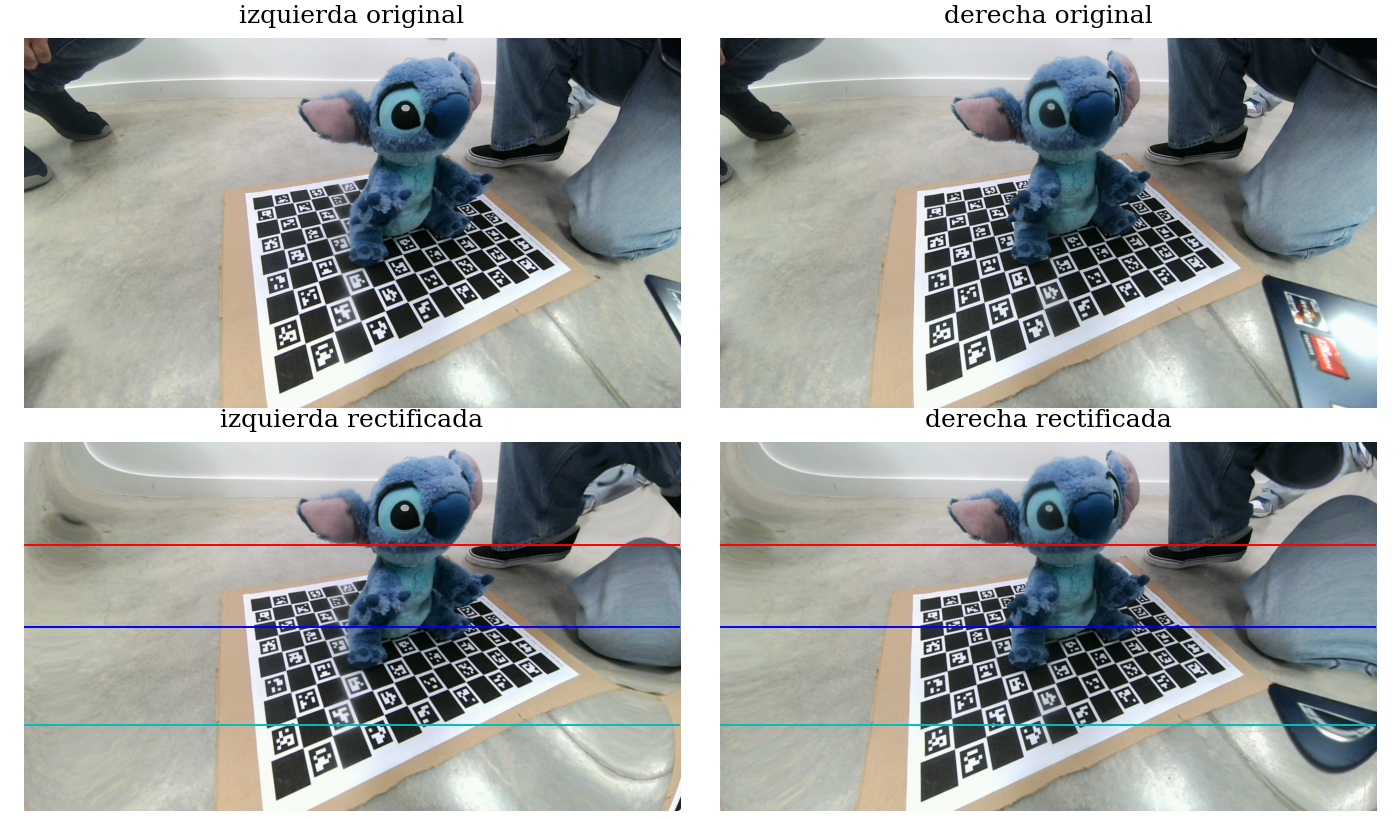
\includegraphics[width=0.62\textwidth]{rectificacion.png}
\caption{Par 13 antes (arriba) y después (abajo) de la rectificación. En las imágenes rectificadas los puntos correspondientes se encuentran en la misma fila, lo que se aprecia con las líneas horizontales de referencia.}
\label{fig:rect}
\end{figure*}

\subsection{Disparidad}
\label{sec:res-disp}

La Fig.~\ref{fig:disp} presenta los mapas de disparidad de SGBM para tres pares tomados desde posiciones distintas. El objeto se recupera casi completo y bien separado del fondo, con disparidades de 40 a $110\px$, mientras que el piso muestra el gradiente suave esperable para un plano que se aleja. La fracción de píxeles con disparidad válida es del 48 al 64\,\%; los huecos se concentran en la pared blanca, que carece de textura, en el ojo del peluche, cuyo brillo especular difiere entre ambas cámaras, en las zonas ocluidas para una de las cámaras (por ejemplo, entre los brazos y el cuerpo) y en la franja izquierda de la imagen, donde no existe correspondencia posible.

\begin{figure*}[!t]
\centering
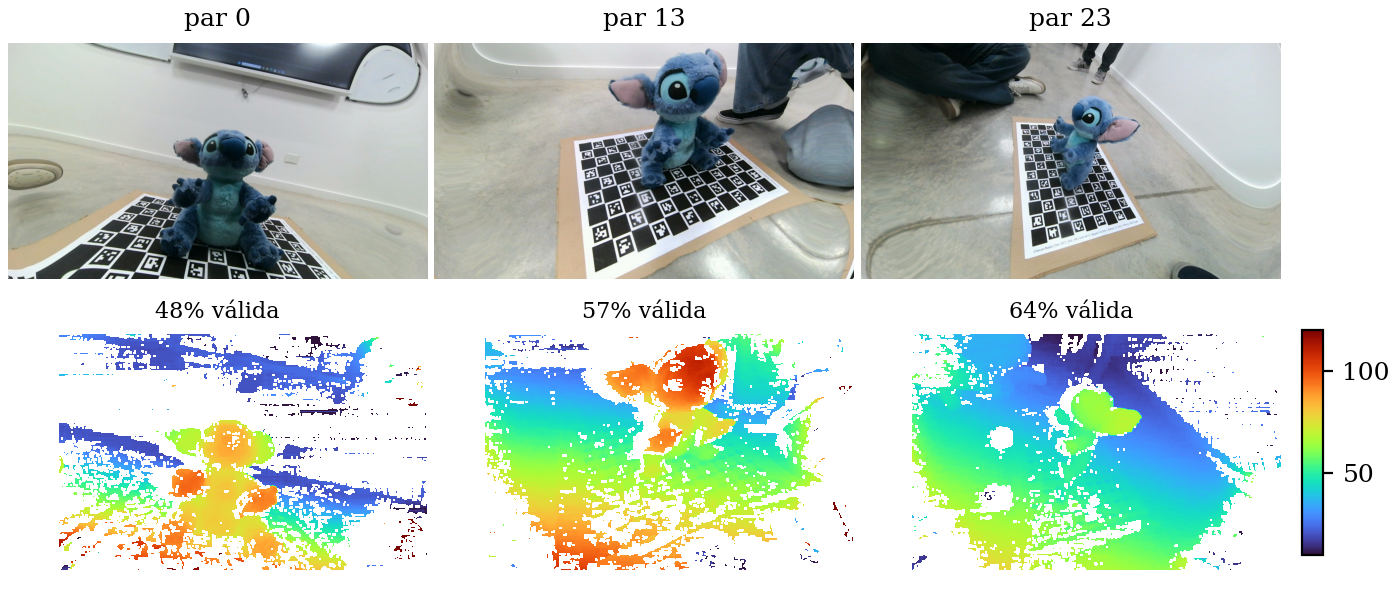
\includegraphics[width=0.72\textwidth]{disparidad.png}
\caption{Arriba: imagen izquierda rectificada de tres pares. Abajo: disparidad calculada con SGBM (en blanco, píxeles sin disparidad válida) y porcentaje de píxeles válidos.}
\label{fig:disp}
\end{figure*}

Como método de \emph{matching} se adoptó \textbf{SGBM}, tras compararlo en \code{stereodemo} con la red neuronal CREStereo sobre el par 13 (Fig.~\ref{fig:metodos}). CREStereo produce un mapa más denso, sin huecos y con contornos nítidos, pero presenta dos desventajas que motivaron su descarte. La primera es el costo: requiere $4{,}9\,\mathrm{s}$ por par, unas 30 veces más que SGBM ($0{,}14$ a $0{,}17\,\mathrm{s}$), aun operando a una resolución reducida de $640\times480$. La segunda, más relevante para una medición métrica, es que asigna disparidad a regiones sin textura, como la pared, en las que no existe información para estimarla: interpola valores plausibles que no provienen de una correspondencia real. SGBM, en cambio, deja esas regiones sin valor, de modo que cada punto de la nube surge de una correspondencia efectivamente observada, y los huecos que deja se cubren con las otras 23 vistas.

Dentro de SGBM, la misma comparación fijó el tamaño de bloque en 5 píxeles. Un bloque de 9 produce un mapa más suave, pero ensancha los bordes del objeto y pierde detalles finos; con 5 se conservan los contornos de las orejas a costa de pequeños huecos, que la redundancia entre vistas compensa. El tiempo de cómputo no depende apreciablemente del tamaño de bloque.

\begin{figure*}[!t]
\centering
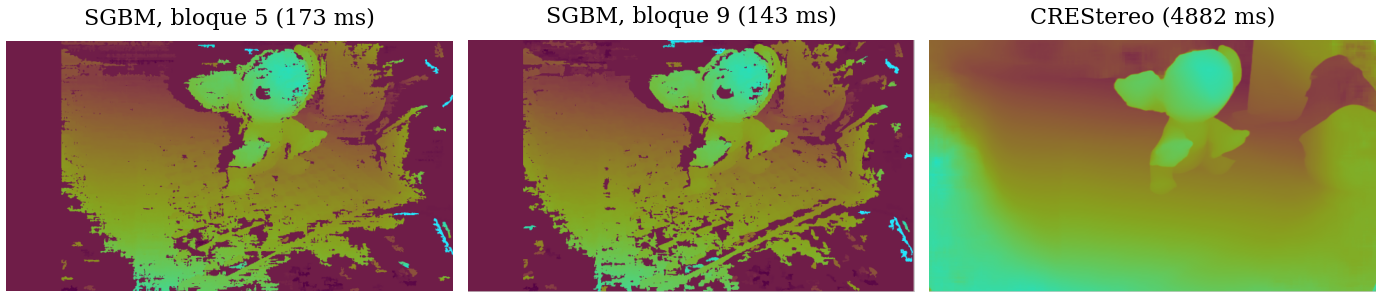
\includegraphics[width=0.75\textwidth]{metodos.png}
\caption{Disparidad del par 13 obtenida en \code{stereodemo} con SGBM (bloques de 5 y 9 píxeles) y con CREStereo, junto con el tiempo de cómputo. El color violeta oscuro indica disparidad no válida en SGBM.}
\label{fig:metodos}
\end{figure*}

\subsection{Nube local, poses y marco global}
\label{sec:res-pose}

La nube local del par 13 contiene $400\,729$ puntos, el 43\,\% de los píxeles (Fig.~\ref{fig:local}). La conversión de \code{reprojectImageTo3D} coincide exactamente con la Ec.~\eqref{eq:depth}: por ejemplo, un píxel con $d=55{,}00\px$ resulta a $Z=444{,}0\mm$. El tablero aparece plano y el peluche se destaca con volumen sobre él, junto con restos del piso y de las personas presentes, que se eliminan en la etapa de fusión.

\begin{figure}[!t]
\centering
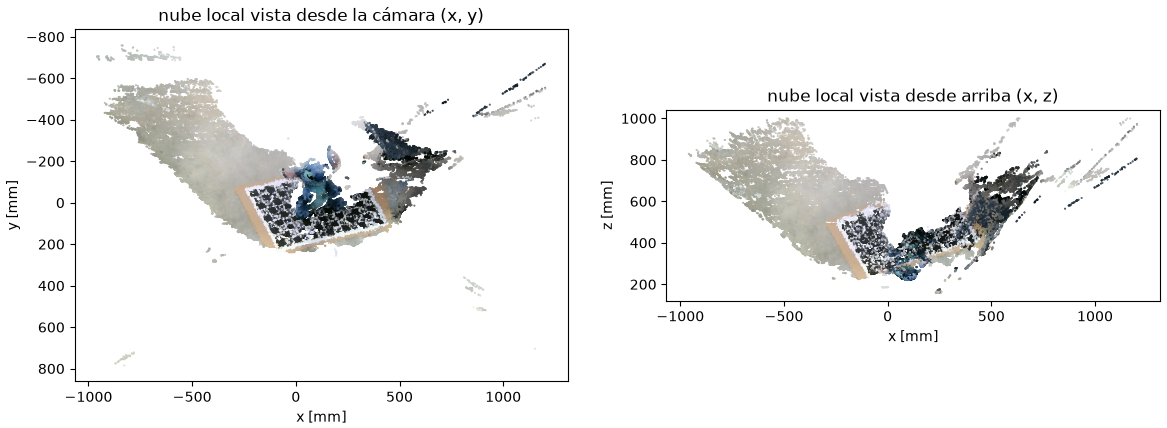
\includegraphics[width=\columnwidth]{nube_local.png}
\caption{Nube local del par 13 en el marco de la cámara izquierda rectificada, vista desde la cámara (izquierda) y desde arriba (derecha).}
\label{fig:local}
\end{figure}

La Fig.~\ref{fig:charuco} muestra la detección del tablero en una de las capturas: aun con el objeto ocluyendo parte del patrón se identifican 32 esquinas y la pose tiene un error de reproyección de $0{,}24\px$. Se aceptaron 24 de los 27 pares: en los pares 1 y 25 no se detectaron suficientes esquinas del tablero (se exigen al menos ocho) y en el par 20 la pose presentó un error de $6{,}1\px$. En los pares aceptados el error de reproyección de PnP estuvo entre $0{,}23$ y $1{,}80\px$. La Fig.~\ref{fig:poses} representa las poses estimadas en el marco global: las cámaras forman una órbita alrededor del tablero, a entre 19 y $55\,\mathrm{cm}$ por encima de su plano, en concordancia con el recorrido realizado durante la captura. La nube del par 13 transformada con la Ec.~\eqref{eq:global} queda correctamente apoyada sobre el tablero.

\begin{figure}[!t]
\centering
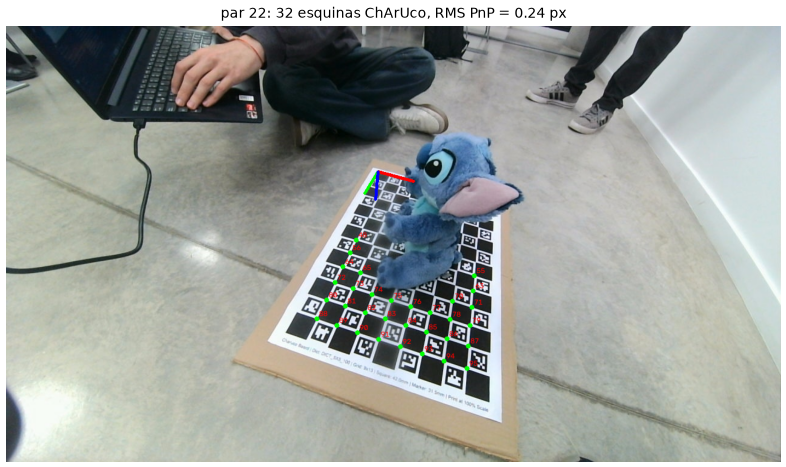
\includegraphics[width=0.92\columnwidth]{charuco_pose.png}
\caption{Esquinas ChArUco detectadas (verde, con su identificador) y ejes del marco global proyectados con la pose estimada (par 22).}
\label{fig:charuco}
\end{figure}

\begin{figure}[!t]
\centering
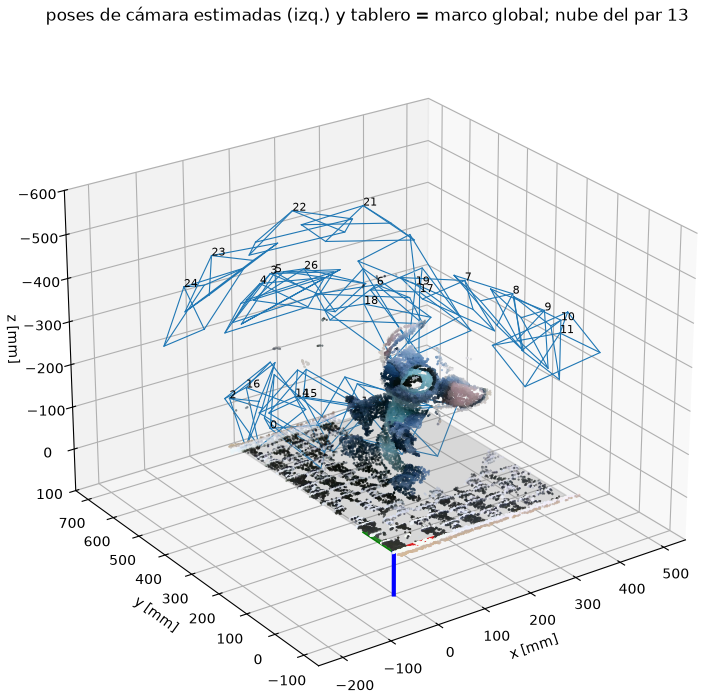
\includegraphics[width=0.95\columnwidth]{poses.png}
\caption{Poses estimadas de la cámara izquierda en el marco del tablero (gris), con su número de par, y nube del par 13 transformada al marco global.}
\label{fig:poses}
\end{figure}

\subsection{Fusión y optimización}
\label{sec:res-fusion}

La Tabla~\ref{tab:fusion} indica la cantidad de puntos que sobrevive a cada etapa y la Fig.~\ref{fig:opt} muestra la nube antes de optimizar, después del filtrado espacial y al final del proceso. La nube global de $9{,}3$ millones de puntos contiene el piso, las personas y el mobiliario del aula; la caja conserva el 16\,\% de los puntos y el submuestreo los reduce a la sexta parte, lo que confirma la gran redundancia entre vistas. El filtrado de outliers elimina pocos puntos, porque los filtros por píxel de la etapa local ya habían descartado la mayoría de los espurios, y la remoción del plano y el agrupamiento separan el tablero y los restos sueltos. La nube final tiene $175\,791$ puntos y el archivo \code{.ply} binario ocupa $4{,}7\,\mathrm{MB}$.

\begin{table}[!t]
\centering\footnotesize
\begin{tabular}{@{}lrr@{}}
\toprule
Etapa & Puntos & Fracción\\
\midrule
Nube global (24 pares) & 9\,282\,487 & 100\,\%\\
1. Caja & 1\,510\,554 & 16,3\,\%\\
2. Vóxeles de 2\,mm & 239\,309 & 2,6\,\%\\
3. Outliers (estadístico + radio) & 233\,096 & 2,5\,\%\\
4. Sin plano del tablero & 180\,711 & 1,9\,\%\\
5. Componente principal (final) & 175\,791 & 1,9\,\%\\
\bottomrule
\end{tabular}
\caption{Puntos que sobreviven a cada etapa de la optimización.}
\label{tab:fusion}
\end{table}

\begin{figure}[!t]
\centering
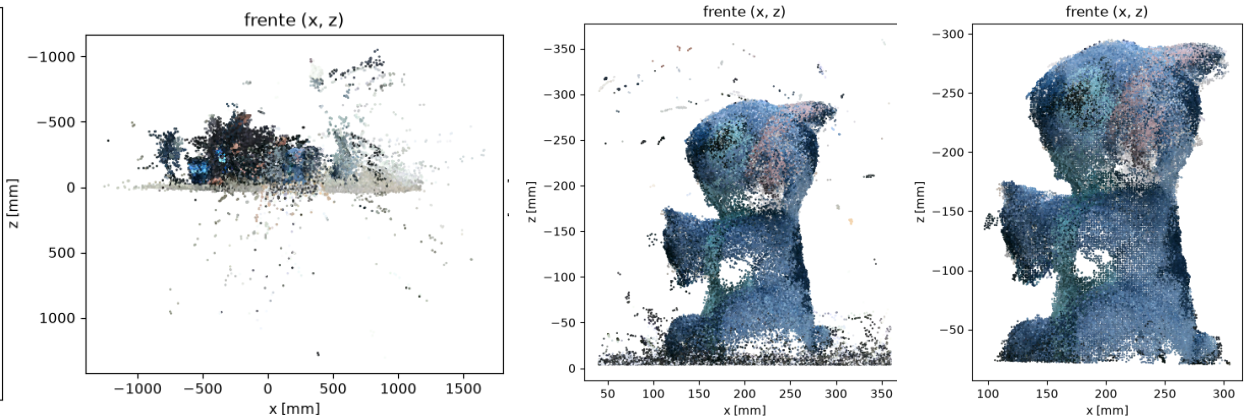
\includegraphics[width=\columnwidth]{optimizacion.png}
\caption{Vista frontal ($x$--$z$) de la nube global antes de optimizar (izquierda; nótese la escala), después del filtrado espacial (centro) y al final del proceso (derecha). El eje $z$ crece hacia el interior del tablero.}
\label{fig:opt}
\end{figure}

La Fig.~\ref{fig:meshlab} muestra la nube final abierta en MeshLab, lo que verifica la validez del archivo exportado. La reconstrucción cubre el objeto en sus 360°, incluida la espalda, gracias a que el tablero ChArUco permitió estimar la pose incluso desde los lados en que el peluche lo ocluye parcialmente.

\begin{figure}[!t]
\centering
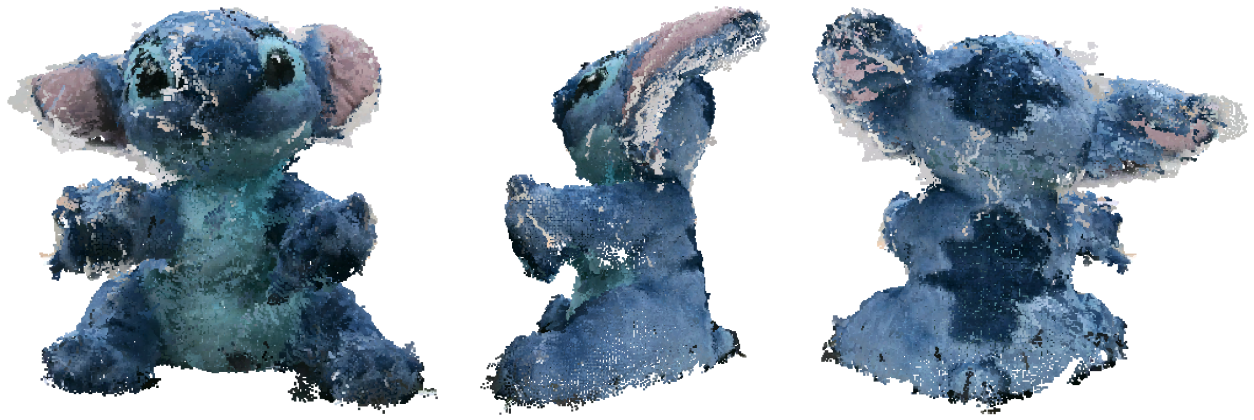
\includegraphics[width=\columnwidth]{meshlab.png}
\caption{Nube final optimizada visualizada en MeshLab: vistas frontal, lateral y posterior.}
\label{fig:meshlab}
\end{figure}

\subsection{Malla de Poisson}
\label{sec:res-poisson}

La Fig.~\ref{fig:poisson} muestra la malla obtenida, de $74\,102$ vértices y unos $150\,000$ triángulos, exportada como un archivo \code{.ply} aparte de $5{,}7\,\mathrm{MB}$. La malla recupera la forma completa del objeto, incluida la espalda, y se mantiene próxima a los datos: la distancia de cada vértice al punto más cercano de la nube tiene una mediana de $1{,}0\mm$ y un percentil 95 de $2{,}0\mm$, del orden del tamaño de vóxel. La vista sombreada pone de manifiesto una superficie rugosa, porque la malla reproduce el ruido de la nube (el pelaje y el leve engrosamiento debido a la fusión de vistas), que el suavizado atenúa pero no elimina. Además, la malla no es cerrada: la base y el hueco entre el brazo y el cuerpo, que ninguna cámara observó con claridad, quedan abiertos porque el recorte por densidad elimina la superficie que Poisson completa sin datos que la sustenten. La medición de la sección siguiente se realizó sobre la nube de puntos, no sobre la malla.

\begin{figure}[!t]
\centering
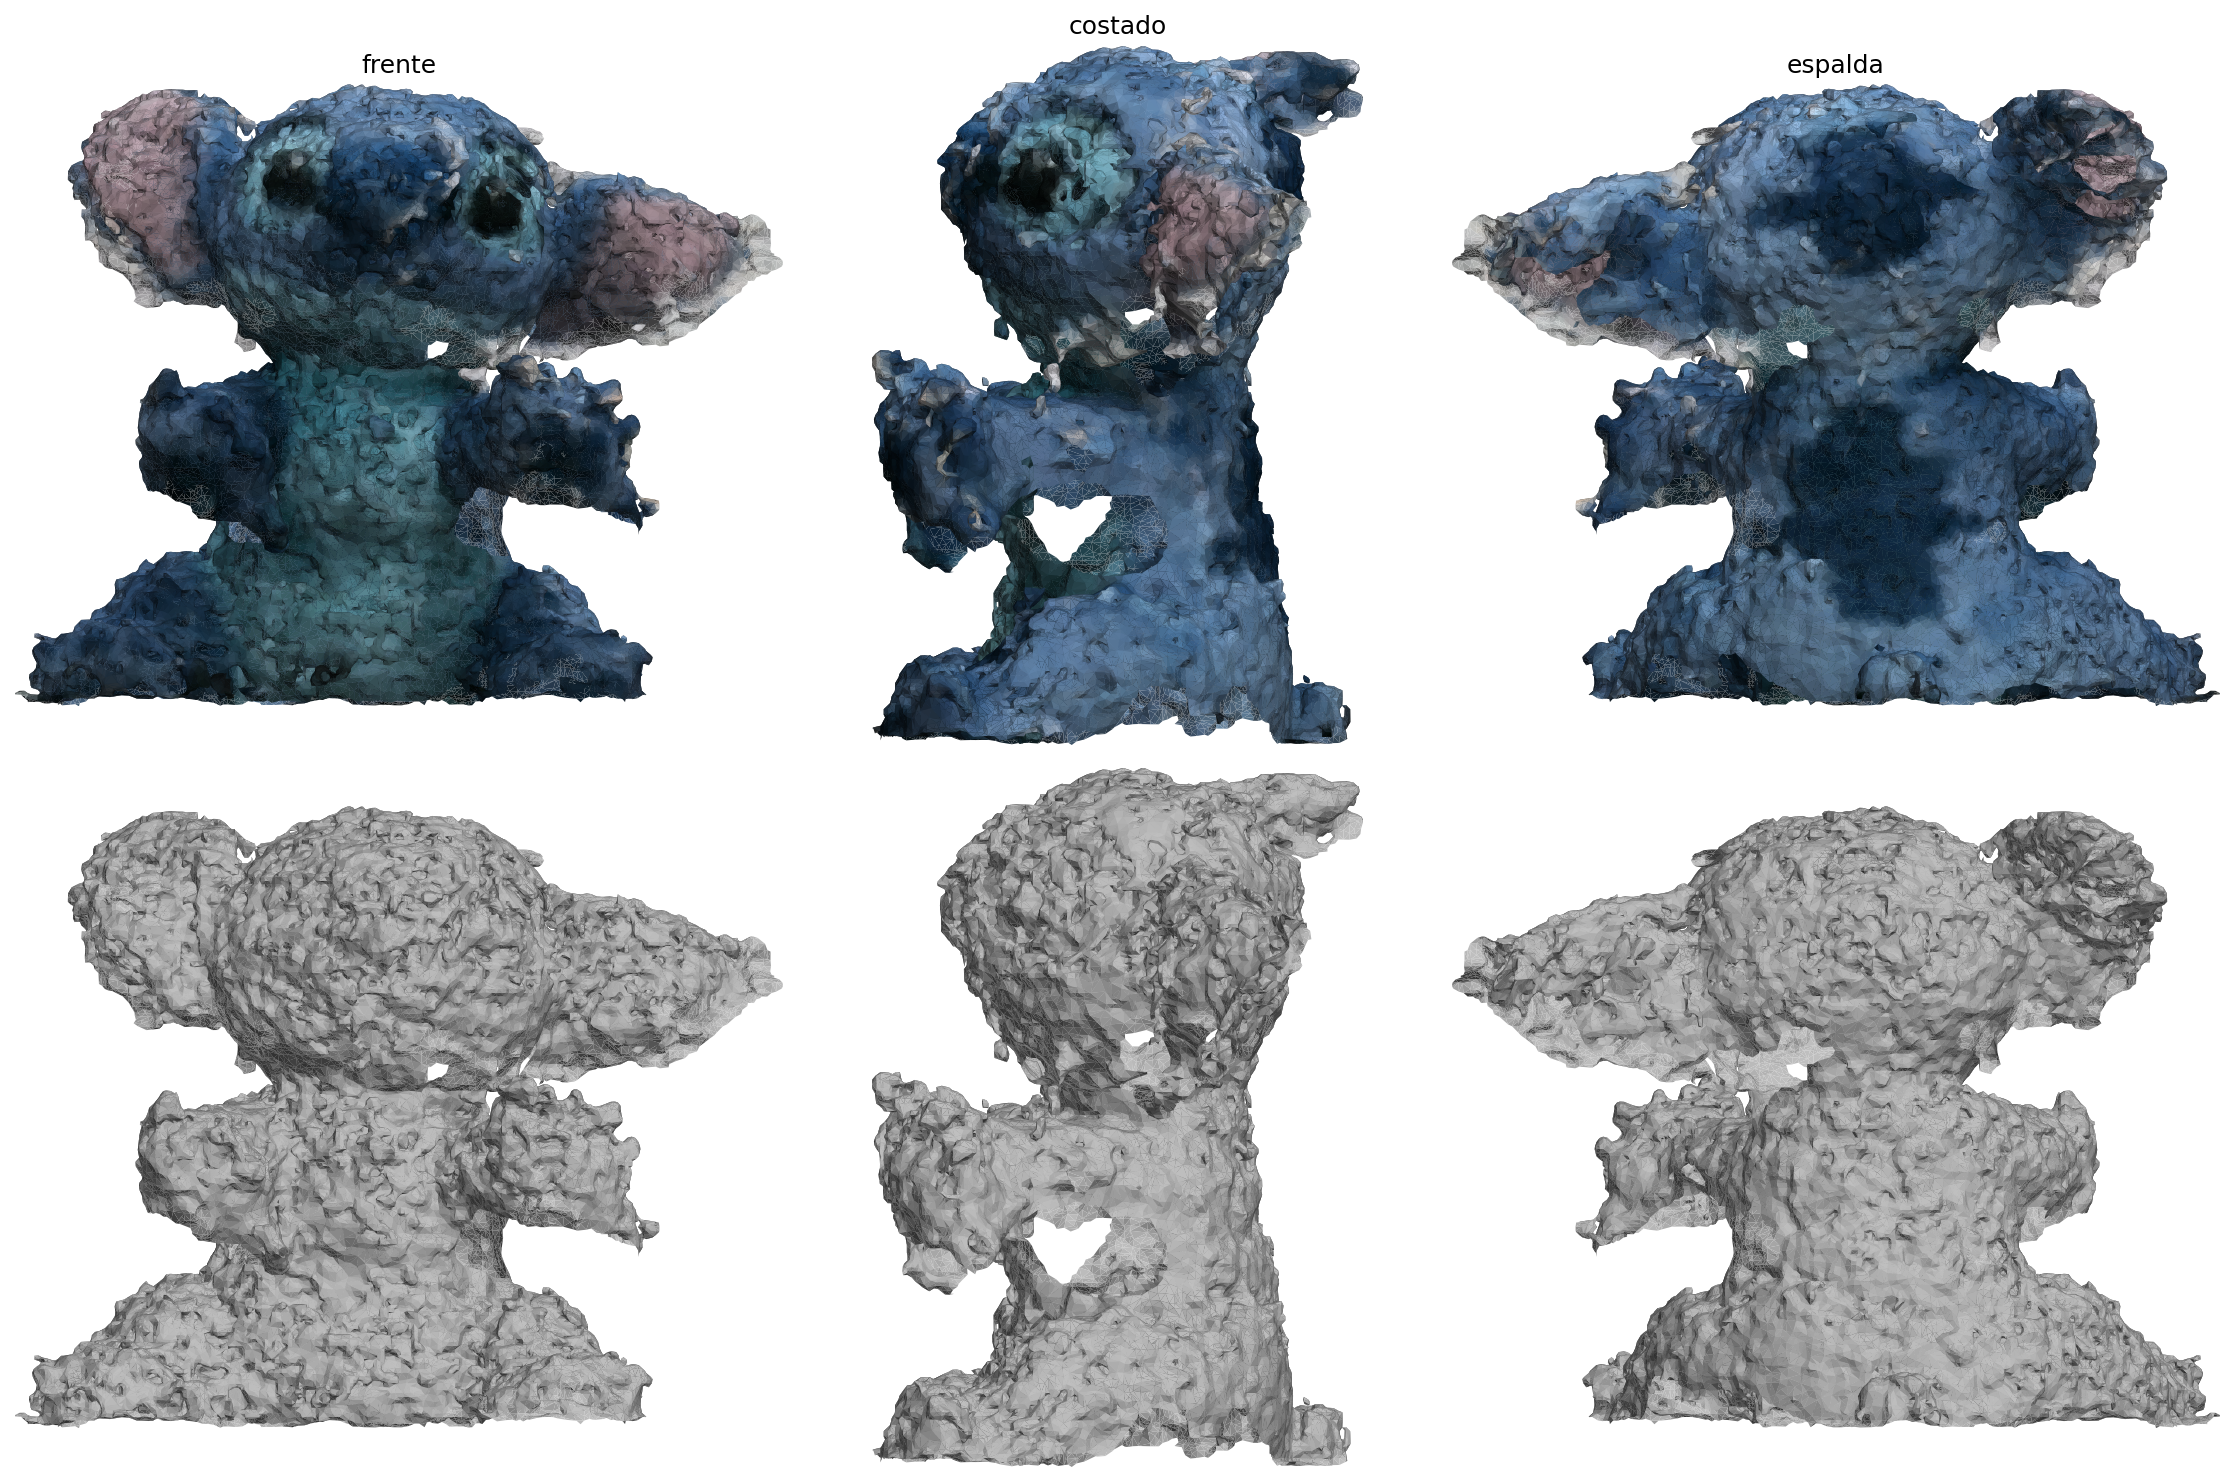
\includegraphics[width=\columnwidth]{poisson.png}
\caption{Malla obtenida con la reconstrucción de Poisson, vista de frente, de costado y de espalda: con el color de la nube (arriba) y en gris con sombreado (abajo), que deja ver la geometría.}
\label{fig:poisson}
\end{figure}

\subsection{Medición métrica}
\label{sec:res-medicion}

Sobre la nube final se obtuvo un \textbf{alto de $279{,}7\mm$} (máximo $286{,}0\mm$), un \textbf{ancho de $294{,}0\mm$} entre las puntas de las orejas y una profundidad de $172{,}5\mm$ (Fig.~\ref{fig:medicion}). Medido con regla, el peluche tiene un alto de $290\mm$, un ancho de $300\mm$ y una profundidad de $170\mm$, por lo que los errores relativos son de $-3{,}5$\,\%, $-2{,}0$\,\% y $+1{,}4$\,\%, respectivamente. El alto y el ancho resultan algo menores que los reales por dos motivos. Por un lado, la medición descarta a propósito los extremos: el alto es el percentil 99,5 de la distancia al plano (con el máximo, $286{,}0\mm$, el error se reduce a $-1{,}4$\,\%) y el rectángulo encierra el 99\,\% central de la huella, por lo que se pierden las puntas de las orejas. Por otro, el filtro de bordes de profundidad y la eliminación de outliers descartan los puntos más dispersos del contorno, que es justamente donde está el pelaje que la regla sí alcanza.

\begin{figure}[!t]
\centering
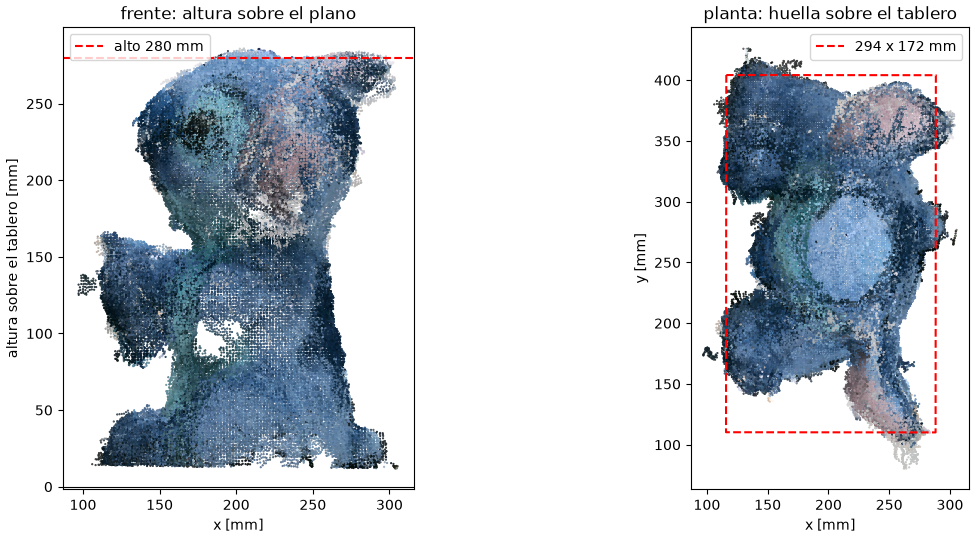
\includegraphics[width=\columnwidth]{medicion.png}
\caption{Medición sobre la nube final. Izquierda: altura de cada punto sobre el plano del tablero y alto estimado (percentil 99,5). Derecha: huella sobre el tablero y rectángulo de área mínima.}
\label{fig:medicion}
\end{figure}

\subsection{Discusión}
\label{sec:discusion}

El pipeline produce una reconstrucción completa y métrica del objeto, pero el análisis de los resultados intermedios pone de manifiesto varias limitaciones.

\textbf{Calibración y rectificación.} El desfasaje vertical residual de $0{,}2$ a $1{,}5\px$ entre imágenes rectificadas tiene siempre el mismo signo, lo que indica un error sistemático de la calibración y no ruido de detección. Que sea mayor cuando el tablero está en el borde de la imagen sugiere que el modelo de distorsión está peor determinado en esa zona, por falta de vistas de calibración que la cubran. SGBM busca correspondencias sólo en la misma fila, por lo que este desfasaje degrada el \emph{matching} en los bordes; recalibrar con más vistas en las esquinas del campo visual permitiría reducirlo.

\textbf{Consistencia entre escalas.} El plano del tablero reconstruido por estéreo quedó $10{,}4\mm$ por encima del plano $z=0$ que define la pose de PnP, alrededor del 2\,\% de la distancia de trabajo. Ambas mediciones son métricas pero no exactamente consistentes: la profundidad estéreo depende de $f$, $B$ y de la rectificación, mientras que la pose depende de los intrínsecos de la cámara izquierda y del tamaño del tablero, y los errores residuales de calibración afectan a cada una de manera distinta. Por esta razón el alto se midió respecto del plano ajustado, lo que cancela el sesgo. Al fusionar vistas desde distintas direcciones, este tipo de error se traduce en un leve engrosamiento de las superficies.

\textbf{Disparidad.} La resolución en profundidad empeora con la distancia según $\delta Z=Z^2\delta d/(fB)$: un error de un píxel de disparidad equivale a $3{,}7\mm$ a $30\,\mathrm{cm}$ y a $12\mm$ a $55\,\mathrm{cm}$, de modo que las vistas cercanas aportan los puntos más precisos. Los huecos debidos al brillo del ojo y a las oclusiones se compensan sólo parcialmente con otras vistas; persiste, por ejemplo, un hueco entre el brazo y el cuerpo, que ninguna cámara observó con claridad. Los métodos basados en redes neuronales, como CREStereo, completarían esas zonas a un costo de cómputo mucho mayor y con el riesgo de introducir estructura inexistente.

\textbf{Puntos espurios.} En el contorno de las orejas se observan puntos de color gris, provenientes del fondo, que el filtro de bordes de profundidad no eliminó por completo: son \emph{flying pixels} en los que la disparidad varía de forma gradual. También sobreviven restos del tablero bajo la base del objeto, cerca del umbral de $10\mm$ de la remoción del plano, que a su vez elimina los últimos milímetros de la base.

\textbf{Poses.} El par~19 se aceptó con una pose menos confiable (error de reproyección de $1{,}80\px$, tras descartar 12 de 38 esquinas). El par~1 se encuentra en el límite de detección: según la versión de OpenCV se detectan 10 esquinas, y el par se acepta, o menos de ocho, y se descarta. Incluirlo o no modifica el alto en sólo $0{,}2\mm$ ($279{,}9$ frente a $279{,}7\mm$), lo que indica que el resultado no depende de pares individuales. Un refinamiento de las poses con ICP entre nubes vecinas, o una optimización conjunta de todas ellas, reduciría el efecto de los pares menos confiables y del sesgo entre escalas.

\textbf{Conclusión.} El sistema estéreo calibrado, junto con el tablero ChArUco como referencia común, permitió reconstruir el objeto en sus 360° y medirlo con escala métrica: el lado del casillero se recupera con un error del $0{,}3$\,\% y las dimensiones del objeto, con errores relativos de $3{,}5$\,\% en el alto y $2{,}0$\,\% en el ancho respecto de las medidas reales. La reconstrucción de Poisson permitió además obtener una superficie continua, fiel a la nube dentro de unos $2\mm$. Como mejoras se proponen recalibrar cubriendo mejor los bordes del sensor y refinar las poses con ICP, lo que reduciría el engrosamiento de las superficies y, con él, la rugosidad de la malla.

\begin{thebibliography}{99}\footnotesize\setlength{\itemsep}{0pt}\setlength{\parsep}{0pt}
\bibitem{hz} R. Hartley y A. Zisserman, \emph{Multiple View Geometry in Computer Vision}, 2.ª ed., Cambridge University Press, 2004.
\bibitem{zhang} Z. Zhang, ``A flexible new technique for camera calibration'', \emph{IEEE TPAMI}, 22(11):1330--1334, 2000.
\bibitem{sgbm} H. Hirschmüller, ``Stereo processing by semiglobal matching and mutual information'', \emph{IEEE TPAMI}, 30(2):328--341, 2008.
\bibitem{crestereo} J. Li et al., ``Practical stereo matching via cascaded recurrent network with adaptive correlation'', \emph{CVPR}, 2022.
\bibitem{aruco} S. Garrido-Jurado et al., ``Automatic generation and detection of highly reliable fiducial markers under occlusion'', \emph{Pattern Recognition}, 47(6):2280--2292, 2014.
\bibitem{ippe} T. Collins y A. Bartoli, ``Infinitesimal plane-based pose estimation'', \emph{IJCV}, 109(3):252--286, 2014.
\bibitem{open3d} Q.-Y. Zhou, J. Park y V. Koltun, ``Open3D: A modern library for 3D data processing'', \emph{arXiv:1801.09847}, 2018.
\bibitem{dbscan} M. Ester et al., ``A density-based algorithm for discovering clusters in large spatial databases with noise'', \emph{KDD}, 1996.
\bibitem{poisson} M. Kazhdan, M. Bolitho y H. Hoppe, ``Poisson surface reconstruction'', \emph{Eurographics Symposium on Geometry Processing}, 2006.
\bibitem{taubin} G. Taubin, ``A signal processing approach to fair surface design'', \emph{SIGGRAPH}, 1995.
\end{thebibliography}

\end{document}
